\chapter{Applicazioni}
\section{Sistemi di Equazioni Differenziali}
Fin ora sono stati tratti solo problemi di Cauchy del primo ordine, del tipo \ref{ode}. Il più delle volte però si è costretti ad analizzare equazioni differenziali di ordine superiore al primo:
\begin{equation}
	y^n(t) = f(t, y(t), y'(t), y''(t),...,y^{n-1}(t))
\end{equation}
con $n-1$ condizioni iniziali.
\\Introducendo delle variabili ausiliarie:
\begin{equation*}
	z_1(t) = y(t) \quad z_2(t) = y'(t) \quad ... \quad z_N(t) = y^{n-1}(t)
\end{equation*}
si può ottenere una equazione differenziale del primo ordine equivalente:
\begin{equation*}
	\textbf{z}'(t) = \begin{pmatrix}
		z_1'(t) \\ z_2'(t) \\ \vdots \\ z_n'(t)
	\end{pmatrix}
 	= \begin{pmatrix}
 		y'(t) \\ y''(t) \\ \vdots \\ y^{n}(t)
 	\end{pmatrix}
 	= \begin{pmatrix}
 		z_2(t) \\ z_3(t) \\ \vdots \\ f(t, z_1(t), z_2(t), ..., z_n(t))
 	\end{pmatrix}
 	= \textbf{g}(t, \textbf{z}(t))
\end{equation*}
A questo punto si può applicare il metodo di Eulero alla variabile $\textbf{z}(t)$ multidimensionale.
\begin{example}
	Sia il seguente problema di Cauchy:
	\begin{equation*}
		x''(t) = -\lambda x(t)
	\end{equation*}
	con $x(0) = 0$ e $x'(0) = 0$
	Utilizzando $\textbf{v}(t)$ come variabile ausiliaria:
	\begin{equation*}
		\textbf{v}(t) = \begin{pmatrix}
			x(t) \\ x'(t)
		\end{pmatrix}
		= \begin{pmatrix}
			v_1(t) \\ v_2(t)
		\end{pmatrix}
	\end{equation*}
	La nuova equazione differenziale diventa:
	\begin{equation*}
		\textbf{v}'(t) = \begin{pmatrix}
			x'(t) \\ x''(t)
		\end{pmatrix}
		= \begin{pmatrix}
			v_2(t) \\ -\lambda v_1(t)
		\end{pmatrix}
	 	= \textbf{g}(t, \textbf{v}(t))
	\end{equation*}
	in cui $\textbf{g}(t)$ è la nuova funzione vettoriale che descrive $\textbf{v}'(t)$
\end{example}
L'implementazione in MATLAB prevede un cambiamento rispetto alla normale implementazione descritta in precedenza.
\\I parametri di ingresso alla funzione sono:
\begin{itemize}
	\item \textbf{$f$} Funzione vettoriale dell'equazione differenziale di tipo \ref{ode}
	\item \textbf{$y_0$} Vettore delle condizioni iniziali al tempo $t_0$
	\item \textbf{$t_0$} Tempo iniziale
	\item \textbf{$T$} Tempo finale
	\item \textbf{$h$} Passo di discretizzazione
\end{itemize}
I parametri in uscita sono:
\begin{itemize}
	\item \textbf{$t$} Asse dei tempi discretizzato
	\item \textbf{$y$} Matrice soluzione soluzione
\end{itemize} 
La soluzione $y(t)$ viene vista come un vettore di vettori. Definito il passo di discretizzazione $h$ e, quindi, $N$ numero di intervalli, la dimensione della soluzione è $n\times N$ (con $n$ ordine dell'equazione differenziale).
\begin{minted}[framesep = 1mm,
	fontsize = \footnotesize,
	]{MATLAB}
function [y, t] = eulero32(f, y0, t0, T, h)
	t = single(t0:h:T);                 %Asse dei tempi discretizzata con passo h
	y = single(zeros(length(y0),length(t)));     %Vettore soluzione
	y(:,1) = y0;                  %Condizione iniziale
	
	for i=1:length(t)-1
		y(:,i+1) = y(:,i) + f(t(i), y(:,i))*h;    %Costruzione della soluzione
	end
end
\end{minted}
\begin{minted}[framesep = 1mm,
	fontsize = \footnotesize,
	]{MATLAB}
function [y, t] = eulero64(f, y0, t0, T, h)
	t = t0:h:T;                 %Asse dei tempi discretizzata con passo h
	y = zeros(zeros(length(y0),length(t));     %Vettore soluzione
	y(:,1) = y0;                  %Condizione iniziale
	
	for i=1:length(t)-1
		y(:,i+1) = y(:,i) + f(t(i), y(:,i))*h;    %Costruzione della soluzione
	end
end
\end{minted}
Il metodo di Eulero viene calcola insieme tutte le soluzioni. Ogni riga rappresenta un vettore soluzione.
\\Questa modifica rende il metodo di Eulero più generale. Infatti una equazione differenziale del primo ordine può essere vista come un sistema di equazioni vettoriali con una sola equazione.

\section{Sistema Massa-Molla}
Il sistema massa-molla è un sistema meccanico composto da un corpo di massa $m$, attaccato ad una molla con constante elastica $k$.
\begin{figure}[H]
	\centering   
	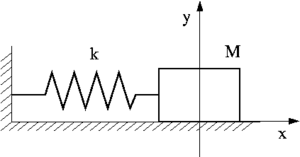
\includegraphics[width=0.5\textwidth]{img/massa-molla.png}
\end{figure} 
Il modello è descritto dalla seguente equazione differenziale:
\begin{equation*}
	m \dfrac{d^2x}{dt^2} = -kx	
\end{equation*}
La soluzione analitica è conosciuta e vale:
\begin{equation*}
	x(t) = A cos(\omega_0t) \quad con \quad \omega_0=\dfrac{k}{m}
\end{equation*}

A questo punto si hanno tutti gli strumenti per analizzare l'errore prodotto dal metodo di Eulero.
\\Si inizia con il calcolo della soluzione numerica per vari $N$:
\begin{minted}[framesep = 1mm,
	breaklines,
	fontsize = \footnotesize,
	]{MATLAB}
%Parametri
k=1;
m=1;

%Condizioni iniziali
t0=0; T=2;
x0=0; v0=1;
y0=[x0,v0];

%Passo di discretizzazione
N = [10^2 10^3 10^4 10^5 10^6 10^7];
h=(T-t0)./N;

%Soluzione anlitica
tempo = t0:h(end):T;
y_analitica = [sin(tempo); cos(tempo)];
plot(tempo, y_analitica(1,:), 'Color', 'Black', 'LineWidth',2);

%Inizializzazione degli errori
gte = zeros(1,length(N));
e_tot = zeros(1, length(N));
e_tot_equivalente = zeros(1, length(N));
roundoff = zeros(1,length(N));
plot(tempo,y_analitica(1,:));

%Soluzione numerica
hold on;
f = @(t,y) [y(2); -k/m*y(1)]; 
for i=1:length(N)
	t = t0:h(i):T;  %Asse dei tempi
	y_numerica = eulero32(f, y0, t0, T, h(i));
	y_numerica_double = eulero64(f, y0, t0, T, h(i));
	roundoff(i) = abs(y_numerica_double(1,end) - y_numerica(1,end));
	e_tot(i) = abs(y_analitica(1,end)-y_numerica(1,end));
	e_tot_equivalente(i) =  abs(y_numerica_double(1,end) - y_numerica(1,end) + y_analitica(1,end)-y_numerica_double(1,end));
	gte(i) = abs(y_analitica(1,end)-y_numerica_double(1,end));
	plot(t,y_numerica(1,:), 'LineWidth', 2);
end
legend('Soluzione Analitica', 'N=10^2', 'N=10^3','N=10^4', 'N=10^5', 'N=10^6', 'N=10^7');
xlabel('Tempo');
ylabel('Soluzione');
grid;
\end{minted}
L'output è il seguente:
\begin{figure}[H]
	\centering   
	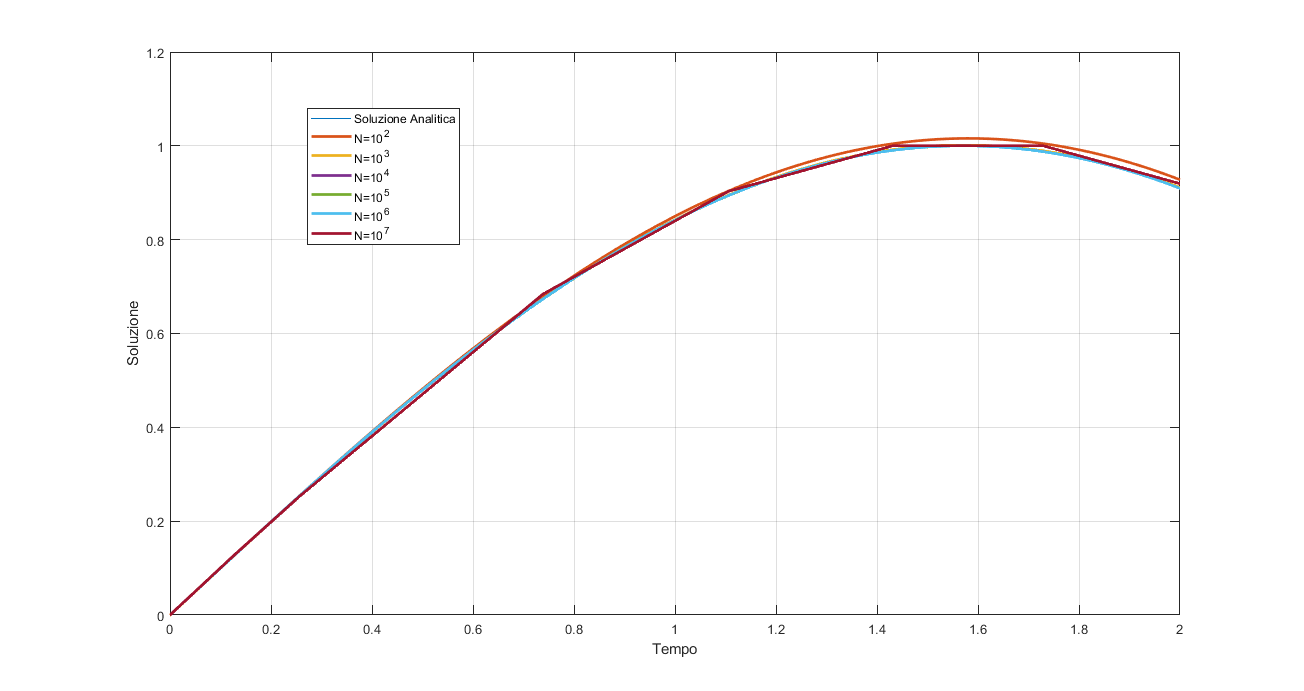
\includegraphics[width=\textwidth]{matlab/esercizio2_soluzioni.png}
	\caption{\textit{Confronto tra le varie soluzioni calcolate}}
\end{figure}
Effettuando uno zoom del grafico si possono notare delle particolarità.
\begin{figure}[H]
	\centering   
	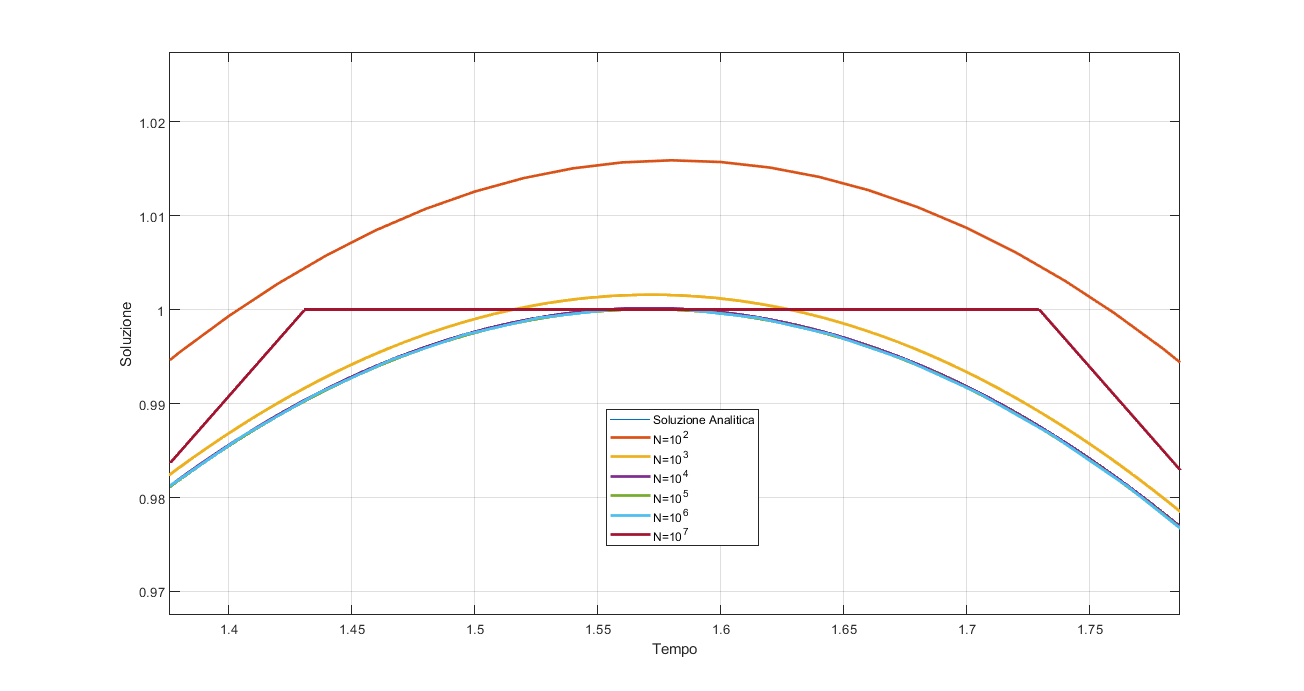
\includegraphics[width=\textwidth]{matlab/esercizio2_soluzioni_zoom1.png}
	\caption{\textit{Zoom delle soluzioni}}
\end{figure}
Già dal grafico si può notare l'influenza dell'errore di roundoff. Infatti per $N=10^7$ l'andamento della soluzione numerica è molto diverso rispetto all'andamento della soluzione analitica.
\\Andando ad effettuare l'analisi degli errori infatti:
\begin{figure}[H]
	\centering   
	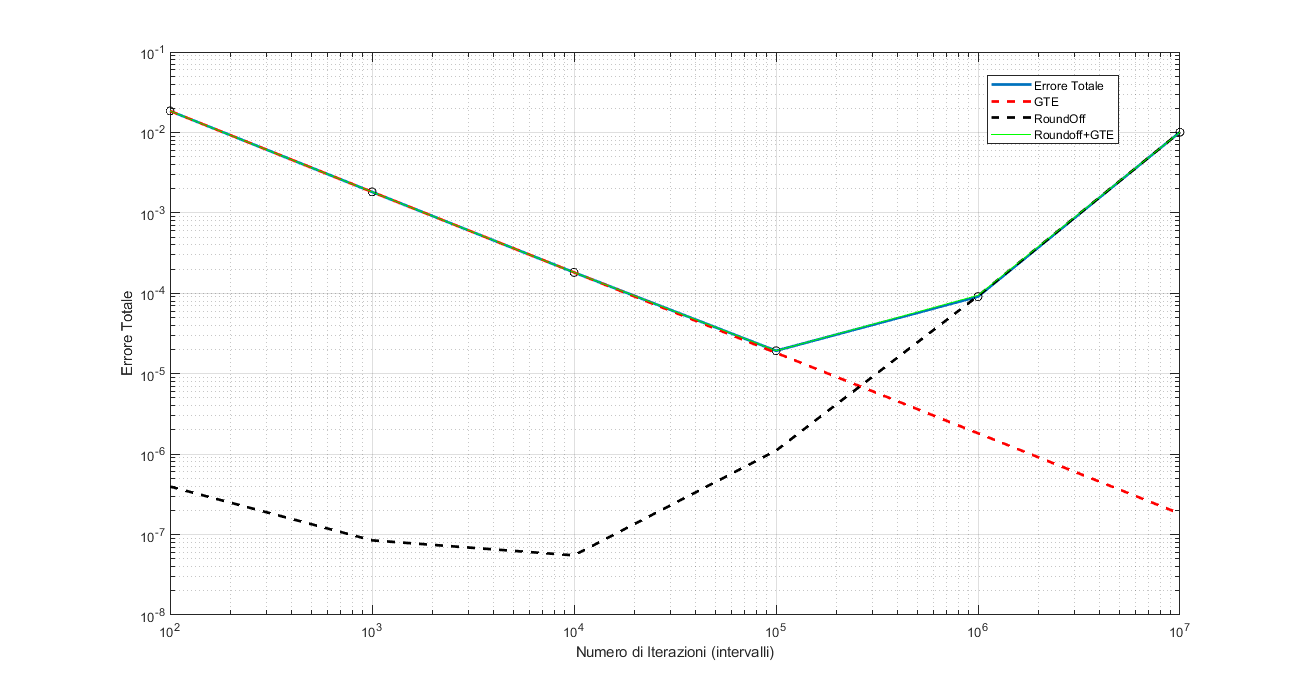
\includegraphics[width=\textwidth]{matlab/esercizio2_errori_confronto.png}
	\caption{\textit{Confronto degli errori}}
\end{figure}
Per $N=10^7$ si ha un errore di $10^{-2}$. 
\\In questo caso il valore di $N$ ottimo è:
\begin{equation*}
	10^5 < N_{opt} < 10^6
\end{equation*}
